\documentclass[9pt,twocolumn,twoside]{../../styles/osajnl}
\usepackage{fancyvrb}
\usepackage{listings}
\usepackage{hyperref}
\usepackage{float}


\journal{i524} 

\title{Deploying a spam message detection application using R over Docker and Kubernetes}

\author[1,*]{Sagar Vora}
\author[1]{Rahul Singh}

\affil[1]{School of Informatics and Computing, Bloomington, IN 47408, U.S.A.}

\affil[*]{Corresponding authors: vorasagar7@gmail.com, rahul\textunderscore singh919@yahoo.com}

\dates{project-P007, \today}

\ociscodes{Docker, Ansible, Kubernetes, R, Pandas, Spam}

% replace this with your url in github/gitlab
\doi{Report: \url{https://github.com/cloudmesh/sp17-i524/tree/master/project/S17-IR-P007/report/report.pdf}\\
Code: \url{https://github.com/cloudmesh/cloudmesh.kubernetes}}
\begin{abstract}
 
Application containerization and automated deployment allows
developers to focus on writing code without worrying about the
environment in which their software is supposed to run. This paper
aims to containerize a standalone R application and deploy it on a
multi node kubernetes cluster and benchmark application performance on
different clouds. Email spam messages are a nuisance to the web
community. If not filtered accurately, they may work like an
email-bomb attack where a stream of spam messages shall make a user to
accidentally omit a legitimate message. We use several established
data mining algorithms to classify messages as legitimate or not, and
compare their classification accuracy. Application and cluster
performance is benchmarked and compared across Chameleon and Kilo
clouds.
\end{abstract}

\setboolean{displaycopyright}{true}

\begin{document}

\maketitle

\section{Introduction}

Email and text messaging are the most formal means of communication
for internet users. Web mining helps any organization to discover
identities of users that it can target to advertise their business by
sending them emails, and at times without their consent. The ease with
which content can be generated and published has also made it easier
to create spam. Spam can be stated as any information which does not
add value to a user of the web. Messages which are inappropriate,
unsolicited, repeated and irrelevant can be all classified as spam. In
this report, we are using data mining algorithms like \emph{SVM
  (Simple Vector Machine)}, \emph{KNN (K-Nearest Neighbor)} and
AdaBoost over an SMS collection dataset of 5574 messages to
differentiate spam messages from legitimate ones. \emph{R} shall be
used to develop the code as it provides supporting text mining
libraries to implement these algorithms.

\noindent

To automate application deployment such that it can be tested on any
environment, docker is used to containerize the application along with
the application dependent libraries. The cluster management tool -
\emph{Kubernetes}, is used to auto deploy the application on a
multi-node cluster. Scripts are written in \emph{Ansible}
\cite{www-ansible} to automate the deployment process. As Kubernetes
itself scales the application container according to our
specification, a deployment engineer shall only be responsible to
write a yaml specificaion file that is read by the kubernetes
engine. Application benchmarking results are achieved by running the
ansible scripts to deploy the application on Chameleon cloud and Kilo
cloud.


\section{ELEMENTS OF THE PROJECT}

\subsection{Ansible}
No one likes repetitive tasks, with Ansible, IT
admins can begin automating away the drudgery from their daily routine
tasks. Ansible is a simple automation language that can perfectly
describe an IT application infrastructure. Ansible is an open source
automation engine which can be used to automate cloud provisioning,
configuration management, and application deployment. It can also
perform more advanced IT tasks such as continuous deployment or
rolling out updates with zero downtime.

A major difference in Ansible and many other tools in the
space is its architecture.

\subsubsection{Architecture}
Ansible is an agentless tool,it doesn't requires any software to be
installed on the remote machines to make them manageable. By default
it manages remote machines over SSH or WinRM, which are natively
present on those platforms \cite{www-ansible-architecture}.

Like other configuration management software, Ansible
distinguishes between two types of servers: one being the controlling
machines and other being the nodes. Ansible uses a single controlling
machine where the orchestration begins. Nodes are then controlled by a
controlling machine over SSH \cite{www-ssh}. The location of the nodes
are described by the inventory of the controlling machine.

Ansible modules are deployed by Ansible over SSH. These modules are
temporarily stored in the nodes and communicate with the controlling
machine through a JSON protocol over the standard output

\subsubsection{Playbooks}

Playbooks \cite{www-ansible-playbook} are Ansible’s configuration,
deployment, and orchestration language. They let us control the remote
systems with a policy which we might want them to enforce. If Ansible
modules act as tools in your workshop, then playbooks are your
instruction manuals, and your inventory of hosts are your raw
material. Playbooks can be used to manage configurations of and
deployments to remote machines. They can sequence multi-tier rollouts
involving rolling updates, and can delegate actions to other hosts,
interacting with monitoring servers and load balancers.

\subsubsection{Ansible Galaxy}

\subsection{R}
R is a language and environment for statistical computing and graphics
\cite{www-about-rproject}. Pandas does not provide a significant
statistical modeling environment as it is still a work in progress. R
provides a variety of statistical model analysis, classification,
clustering and graphical techniques to provide this
environment. Integrating Python's efficiency with R's capability
allows us to build a highly a desirable analysis model for our
application.


\subsection{Docker}

\emph{Docker} is an open-source project that automates application
deployment by packaging the application in
\emph{containers}. Containers provide application portability by
bundling together an application and its needed resources in a package
so that they can be deployed on different platforms without worrying
about resource dependencies. Application containerization is an OS
(Operating System) level emph{virtualization} for deploying and
running an application instance without launching a virtual mahine for
each application \cite{www-containerization}. A container has its own
environment variables, filesystem and libraries that is needed by the
application, thus eliminating OS or hardware dependency. Containers
abstract the OS kernel while a \emph{VM (Virtual Machine)} hypervisor
abstracts an entire device.

Docker allows application developers to package their applications
into isolated containers. Docker automates the repetitive tasks of
setting up and configuring development environments thus allowing
developers to focus only on building software. A dockerized
application can simply ship between platforms as the complexity of
software dependencies is handled by the container.  Docker
standardizes container creation and can be used to pack, ship and run
an application as a lightweight container that can run in any
environment. Docker can be integrated with other devops applications
like Puppet, Chef, Vagrant, Ansible and Kubernetes. We shall use
Docker with Ansible and Kubernetes in our project.

\subsubsection{Dockerfile and DockerImage}
To package an application and its dependencies in a single file,
docker introduces the concept of a \emph{docker image}. The docker
engine creates a docker image by parsing contents of a
\emph{dockerfile}. A dockerfile is a script composed of various
commands to build a container in a step-by-step, layer-by-layer manner
\cite{www-docker-digitalocean}. Once an image has been built it can be
shared with other users by pushing it to a public repository on
\emph{DockerHub} or \emph{GoogleCloudPlatform}. In this manner, an
image once built by the docker engine can be used across the
organization by making a docker pull request.

\subsection{Kubernetes}
Kubernetes is an open-source platform for automating deployment,
management and scaling of containerized applications across a cluster
\cite{www-wiki-kubernetes}. The more granular an application is, the
more components it consists of and thus requires management of these
components. Kubernetes helps in faster deployment of applications and
scaling them on the fly. Moreover it optimizes the use of hardware by
using the resources which are needed. Kubernetes provides container
management features like component replication, load-balancing,
service-discovery and logging across components
\cite{www-kubernetes-architecture}. A Kubernetes cluster can be
deployed on either physical or virtual machines. We shall be deploying
a kubernetes cluster using \emph{kubeadm} - the kubernetes command
line tool and \emph{Minikube} which is a lightweight Kubernetes
implementation which creates a VM on the local machine and deploys a
simple cluster containing only one node. The Minikube CLI provides
basic bootstrapping operations for working with the cluster, including
start, stop, status, and delete commands.

\subsection{Kubernetes Terminologies}
Kubernetes defines the following set of primitives which provide
mechanisms for deploying and scaling applications.

\subsubsection{Pods}
A pod is the smallest unit of a kubernetes cluster and has a unique
ip-address within the cluster. A pod consists of one or more
containers that can share resources and can be controlled as a single
application \cite{www-wiki-kubernetes}
\cite{www-kubernetes-digitalocean}. Thus all the involved containers
in a pod are scheduled on the same host. A pod can be thought of as a
single virtual machine in terms of resource sharing and scheduling.
Pods can be managed manually using the \emph{Kubernetes API} or can be
managed by a controller.

\subsubsection{Services}
A kubernetes service is a collection of pods that perform the same
function and are presented as a single entity. This way a service can
be emphasized as a one tier of a multi-tier application. Service act
as an interface to a group of containers so that service-consumers
need only reference the single access location. Kubernetes facilitates
service discovery by assigning a stable IP address and a namespace to
a service. This idea abstracts the change of IP addresses of pods
within a service that result due to pod failure or pod rescheduling.

\subsubsection{Replication Controllers}
A replication controller is a framework for horizontal scaling of
pods. Semantics of a pod are defined in a <pod\textunderscore
name>.yaml file which also defines the replication details that need
to be done. The replication controller performs replication by scaling
a number of pods across a cluster based on the pod definition file
\cite{www-wiki-kubernetes}. The replication controller has to make
sure that a certain number of copies of a pod are always up and
running. Thus, in event of a pod failure it replaces the failed pod
with a new replica.

\subsubsection{Labels and Selectors}
Kubernetes allows users or internal components to assign a key-value
pair tag to any API object in the system. An object can have one or
more labels associated with it, but each with a unique key. eg:
appversion = 1.0, development\textunderscore stage = 4.  Label
selectors are queries against labels that return matching objects
\cite{www-kubernetes-digitalocean}. This way each object in the system
can be referenced with a single label or a combination of multiple
labels for fine grained control.

\subsection{Kubernetes architecture}
Kubernetes exhibits the master-slave architecture. The components can
be split into those that manage an individual node(slave) and those
that manage the master or control plane.

\begin{figure}[htbp]
\centering
\fbox{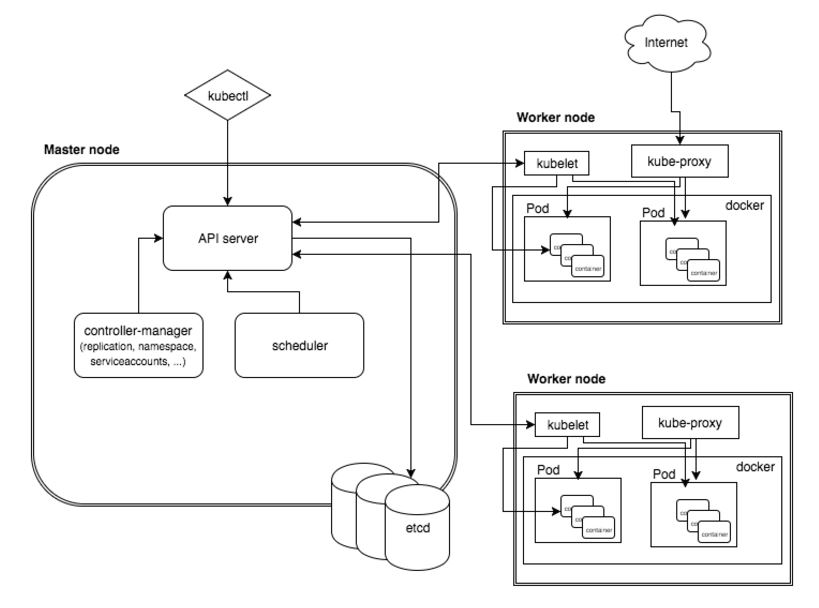
\includegraphics[width=60mm,height=60mm]{images/kubernetesArchitecture.JPG}}
\caption{Kubernetes architecure \cite{www-kubernetes-architecture}}
\label{fig:Kubernetes Minimum Architecture}
\end{figure}


\textbf{Kubernetes Master Node/Control plane}
\newline
The Kubernetes master node is responsible for managing the kubernetes
cluster and orchestrating the worker nodes, where the actual pods are
scheduled. The master node can work as a single node cluster where it
can schedule pods to work on the master node itself by tainting the
schedule policy rule on the node. The master node also referred as
the control plane consists of several components:

\subsubsection{API Server}
The API server is the most fundamental component of the Kubernetes
master and serves as the entry point for all the REST commands used to
control the cluster. The API server serves up the Kubernetes API using
JSON over HTTP, providing both internal and external interface to the
cluster \cite{www-kubernetes-digitalocean}
\cite{www-apiserver-kmblog}. It validates the REST requests, executes
them and updates the status of the objects in the \emph{etcd} storage.

\subsubsection{etcd storage}
\emph{etcd} is a simple, distributed and consistent key-value store
that stores configuration data of the cluster and represents the state
of the cluster at any point of time
\cite{www-wiki-kubernetes}. Kubernetes uses etcd for service discovery
and provides a simple HTTP/JSON API as an interface for setting or
retrieving values from the store. Other components watch the state of
the etcd store to bring themselves up to the desired state. Data being
stored in the etcd store are deployed services, pods, replication
information etc.

\subsubsection{Scheduler}
The scheduler component is responsible for the deployment of pods and
services on the cluster nodes. The scheduler has the information about
the availability of resources on a node and schedules unscheduled pods
on the nodes accordingly. Along with scheduling, the scheduler also
tracks resource utilization of each node and ensures that workload
scheduled is not in excess to the resources available
\cite{www-wiki-kubernetes}.

\subsubsection{Controller-manager}
The controller manager is the process embedding the different types of
controllers like the Replication Controller or the DaemonSet
Controller on a kubernetes master. The controllers query the API
Server to manipulate the resources like pods,services etc. which they
manage.

\subsection{Worker Node}
The worker node also called as minion node is where the containers are
actually deployed. The worker contains all the necessary services
needed to manage the networking between containers, communicate with
the master node and assign resources to the scheduled containers
\cite{www-kubernetes-architecture}.  Every worker node must run the
container runtime i.e docker and other components stated below to
ensure proper communication with the master.

\subsubsection{Docker}
Docker runs on each of the worker nodes. It is responsible for
downloading the docker images and running the configured pods by
starting the container.

\subsubsection{Kubelet}
\emph{Kubelet} gets the pod definition from the api-server and is
responsible for maintaining the pod in the desired state. Kubelet is
the worker service that monitors the health of each pod and
communicates the status of each node via a heartbeat message to the
master.  If the pod is not in the desired state, it is redeployed to
the same node \cite{www-wiki-kubernetes}. Kubelet is also responsible
for communicating with the etcd storage to get information about the
services and update the storage about newly created ones.

\subsubsection{Kube-Proxy}
\emph{Kube-proxy} acts as a network proxy and a load balancer. It is
responsible for networking of TCP and UDP packets to the appropriate
container based on the IP address of each packet
\cite{www-wiki-kubernetes} \cite{www-kubernetes-architecture}.

\subsubsection{Kubectl}
\emph{kubectl} is a command line tool that communicated with the API
server to fetch important information about the nodes, pods, services
and events in the cluster.


\section{Design}

\section{About the Application}
We are using a series of machine learning algorithms and shall compare
their perfomance in terms of classifier accuracy. To build our
classifier and check its accuracy, we shall partition the data into 2
subsets - training data and classification data. We shall choose one
of the subsets for training and other for testing and predicting
classifier accuracy.

\subsection{The dataset}
We are using the SMS Spam Collection dataset from UCI's
public machine learning repository to build our classifier. The
dataset consists of 5574 text messages, with each classified as a spam
or ham message \cite{www-sms_spam_collection}.

\subsection{Algorithms Used}

\subsubsection{SVM}
SVM (Support Vector Machines) are discriminative classifier models
that classify the data as belonging to one of the two possible
classes, in our case class ham and class spam. The SVM algorithm
attempts to categorize data by drawing a hyperplane between the data
points such that points on either end of the hyperplane belong to one
of the two possible classes. An SVM model is representation of given
data points in space such that the division between the classes of
data is as clear as possible \cite{www-svm-wiki}. The aim of the algorithm
is to find the optimum hyperplane that defines the largest possible
margin between the classes of data.

\begin{figure}[htbp]
\centering
\fbox{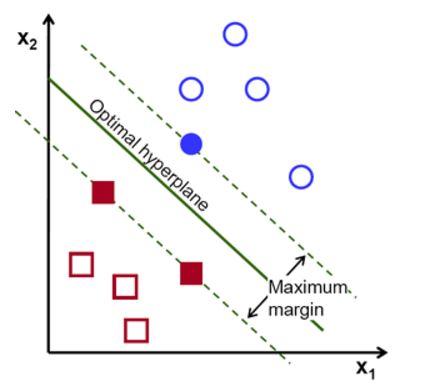
\includegraphics[width=40mm,height=40mm]{images/svm_hyperplane.JPG}}
\caption{The maximum margin hyperplane for SVM \cite{www-svm-tutorial}}
\label{fig:The maximum margin hyperplane for SVM}
\end{figure}

\subsubsection{SVM Kernels}
A simple SVM transfromation works for data with linear decision
boundaries, where the different data points lie on either side of the
decision boundary. But for scenarios where a linear boundary is
efficient to classify data, we need to transform the data from its
original coordinate space into new space so that a linear decision
boundary can be drawn to separate the data in this transformed space
\cite{book-dataminingintroduction}. The kernel is a similarity
function. It is a method to compute similarity between attributes in
the transformed attribute space. We shall use svm kernel methods as
they eliminate the curse of dimensionality problem as they perform the
computations in the original attribute space
\cite{book-dataminingintroduction}. We shall avoid mathematical
details about SVM and the kernel as they are beyond the scope of this
report.

\textbf{Polynomial kernel} - Polynomial kernel, as the name suggests, looks not
only at the given features of the input samples but at their
combination \cite{www-polykernel-wiki}. If a pair of words give
interesting information rather than the individual words alone, we can
use a quadratic kernel. Similarly, for occurences of triplets of
words, we can use a cubic kernel. Linear kernels are special case of
polynomial kernels where the quadratic factor is 1.


\textbf{Radial kernel} - Radial basis kernel maps the data into infinite
dimensional space to extract relations between the variables. It helps
us to draw a circular decision boundaries to pick dependent features.

\subsubsection{K - Nearest Neighbor}
The k-nearest neighbor algorithm classifies a data point as belonging
to either output class by taking a majority vote amongst its k-nearest
neighbors. The algorithm computes distances between the test data
point and all the stored data points or neighbors. \emph{Euclidean
  distance} \cite{www-wiki-euclidean_distance} is used to compute
distance metrics between attribute values of the neighbors. A sample
figure explaining the algorithm is given below.

\begin{figure}[htbp]
\centering
\fbox{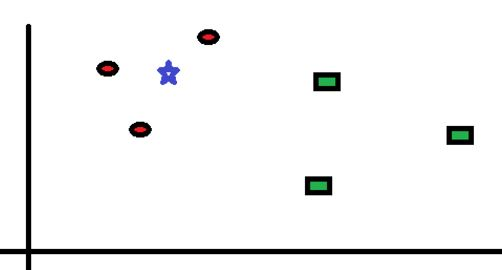
\includegraphics[width=40mm,height=40mm]{images/knn_example.JPG}}
\caption{An example for the K-Nearest Neighbor algorithm \cite{www-knn-introduction}}
\label{fig: An example for the K-Nearest Neighbor algorithm}
\end{figure}

There are 2 classes of data items in the figure - circles and
squares. We have an unknown data point - the star and wish to find its
real class using k-nearest neighbor algorithm. For k=3, the 3-nearest
neighbours according to the distance metrics are all circles. Hence,
the unknown data point is then classified as a circle. This assumption
changes for higher values of k. To eliminate the effect of noise and
outliers on the classification result, a weight is associated with
each data point, with closer neighbors having higher weight over the
distant neighboring points.

\subsubsection{Naive Bayes Classifier}

Naive Bayes classifier works on the principle of conditional
probability. Bayes classifier assigns each sample a probability of
belonging to one class or another. The classifier shall maintain a bag
of words along with the count of each word occuring in the spam
messages. This word count shall be used to calculate and store the
word probability in a table that shall be cross-referenced to
determine the class of the record on classification data
\cite{paper-classification-of-email}.

A selected few words have more probability of occuring in a spam
messages than in the legitimate ones. Eg: The word "Lottery" shall be
encountered more often in a spam message.  The classifier shall
correlate the bag of words with spam and non-spam messages and then
use Bayes Theorem to calculate a probability score that shall indicate
whether a message is a spam or not. The results shall be verified with
the results available on the training dataset and the classifier
accuracy shall be calculated.  The classifier shall use the Bayesian
theorem over the training dataset to calculate probabilities of such
words that occur more often in spam messages and later use a summation
of scores of the occurence of these word probabilities to estimate
whether a message shall be classified as spam or not. After working on
several samples of the training dataset, the classifier shall have
learned a high probability for spam based words whereas, words in
legitimate message like family member or friends names shall have a
very low probability of occurence.

Once the training process has been completed, the posterior
probability for all the words in the new input email is computed using
Bayes theorem. A threshold value shall be defined to classify a
message into either class. A message's spam probability is computed
over all words in its body and if the sum total of the probabilities
exceeds the predefined threshold, the filter shall mark the message as
a spam \cite{www-wiki-naivebayes}.

\subsection{The Classification process}

\subsubsection{Building the classification model}

To address the problem of incoming spam messages, a model shall be
developed using the various classification techniques to correctly
classify each incoming email/text message as a spam or a legitimate
one. The training dataset to build the
model consists of 5574 message records.

To develop an efficient training model, we shall partition the data
into 2 subsets - the training data and testing data. We shall choose
one of the subsets for building a classification model and the other
to evaluate the model's performance. The training process involves
creating a document term matrix for the occurence of each word in the
spam marked messages. This matrix describes the frequency of terms in
each of the messages, with the rows corresponding to documents in the
dataset and columns corresponding to the terms.  Using the document
term matrix, we find highly repeated words in spam messages across the
training set. We vectorize the training and the test data set using
these word frequencies and provide this vectorized data as input to
the various algorithms in our program.

\subsubsection{Testing the model}

Each algorithm used in the application uses its own strategy to build
a classification model from the training set examples. The model's
performance is evaluated by using it to classify the test
dataset. Using the classification results, a confusion
matrix is built to analyze the algorithm's performance on the test dataset.
The confusion matrix specifies what number of spam messages were
correctly classified as spam or incorrectly classified as ham and
vice-versa. Based on these results, we calculate the accuracy of
classification by dividing the number correct results by the total
records in the dataset.

Further, a higher classification accuracy shall be achieved through
filtering by looking at the message header i.e the sender's
number/name. Thereby if a message from a particular sender is
repeatedly marked as spam by the user, the classifier need not
evaluate the message body if it is from the same sender.

\section{DEPLOYMENT}
Our application will be deployed using Ansible \cite{www-ansible}
playbook. Automated deployment should happen on two or more nodes
clouds or on multiple clusters of a single cloud. Deployment script
should install all necessary software along with the project code to
Kubernetes cluster nodes using the Docker image.

\subsection{Deployment process - Ansible}
<TODO - describe the ansible deployment and scripts>

\subsection{Dockerizing the application}
To containerize our application, we need to create a docker image for
it. To create a docker image we need to create a docker file that
describes the semantics to create the docker image. Docker version
used for this process is 1.12.6.

\subsubsection{The Dockerfile}
Docker can build images automatically by reading instructions from a
Dockerfile. A dockerfile is a series of text commands that a user can
run on a command line to build an image \cite{www-dockerfile-documentation}.
\newline
Instructions within a Dockerfile have the following format:
\begin{figure}[H]
\begin{verbatim}
 INSTRUCTION  arguments
\end{verbatim}
\caption{Syntax of every command in a dockerfile}
\label{Syntax of every command in a dockerfile}
\end{figure}

Docker reads the instructions from a dockerfile in the order they are
written. The very first line of a docker file must be a 'FROM' clause
which specifies the base image from which the image is being built. As
our application works with R, we need to specify the base package as
one that shall help us run our R application. \emph{DockerHub} has a
r-base package that binds the latest version of R and its libraries
together that we shall use \cite{www-rbase-docker}.  The argument
following the FROM clause is a repository/tag name that the docker
engine automatically looks up on \url{http://hub.docker.com}.

Following the FROM statement, we can specify all actions we need to
perform like specifying the work directory for building the image or
copying files into our work directory so that every resource is
available under a single folder. Our application needs several text
mining packages to be available as a part of the installation and thus
we use the docker RUN command to download these dependencies and make
them part of the docker image. The R library in the docker container
shall pre-install all the dependencies as the image is built and we
shall only care about running the application logic. Lastly, our
docker file ends with a CMD statement that specifies the command that
the container is supposed to execute on successful instantiation. CMD
accepts an array of command names followed by the parameters. Since we
want our image to execute our R application we shall specify the command
as stated in the dockerfile below.

\begin{figure}[H]
\begin{verbatim}
FROM r-base
COPY . ~/myscripts
WORKDIR ~/myscripts
RUN Rscript -e "install.packages('tm')"
RUN Rscript -e "install.packages('e1071')"
RUN Rscript -e "install.packages('RWeka')"
RUN Rscript -e "install.packages('ada')"
RUN Rscript -e "install.packages('rbenchmark')"
CMD ["Rscript","spamdetection.r"]
\end{verbatim}
\caption{Dockerfile of the application}
\label{Dockerfile of the application}
\end{figure}


\subsubsection{Creating a docker image}

Once the Dockerfile is built, we can build the image using docker
build command as follows :

\begin{figure}[H]
\begin{verbatim}
cc@rahpsing-055:~/dockerDirectory$ sudo docker build 
-t  spamdetectionapplication  ~/dockerDirectory/

Sending build context to Docker daemon  12.8 kB
Step 1 : FROM r-base
latest: Pulling from library/r-base
c560cd7bd403: Pull complete 
b190a5321f19: Pull complete 
3933674049c0: Pull complete 
99d11fb944ea: Pull complete 
34522f7c3788: Pull complete 
c2a798388711: Pull complete 

Digest: sha256:e192edf861d61caff0b329436...
Status: Downloaded newer image for r-base:latest
 ---> 16fe32463daa

Step 2 : COPY . ~/dockerDirectory/
 ---> a6717da2ec47
Removing intermediate container 8fb4aaaec0d8

Step 3 : WORKDIR ~/dockerDirectory/
 ---> Running in 0220b193ed11
 ---> a3c4d57e23c9
Removing intermediate container 0220b193ed11

Step 4 : RUN Rscript -e "install.packages('tm')
       .
       . <installation_logs>
       .
Step 9 : CMD Rscript spamdetection.r
 ---> Running in 4edb44f2ffb6
 ---> a4814eeadf35
Removing intermediate container 4edb44f2ffb6
Successfully built a4814eeadf35
\end{verbatim}
\caption{Building an image line by line from a dockerfile}
\label{Building an image from a dockerfile}
\end{figure}


The built image is placed in our machine's local docker registry and
can be viewed with the 'docker images' command.

\begin{figure}[H]
\begin{verbatim}
$ docker images
REPOSITORY                TAG     IMAGE ID      SIZE
spamdetectionapplication  latest  a4814eeadf  646.1 MB
r-base                    latest  16fe32463d  645.6 MB
\end{verbatim}                   
\caption{Listing images in the local repository}
\label{Listing images in the local repository}
\end{figure}

\subsubsection{Running the application}

We shall run our application using the docker run command.

\begin{figure}[H]
\begin{verbatim}
 docker run spamdetection
\end{verbatim}
\caption{Running a docker image}
\label{Running a docker image}
\end{figure}

We can check the container id of our application along with other
important information using the 'docker ps' command.
 
\subsubsection{Sharing the docker image}

By default, the docker CLI points to docker's public registry which is
located at \url{http://hub.docker.com}. We need to create a docker
account to upload our application image so that it could be directly
referenced by kubernetes later. Once a docker account is registered,
create a public repository and give it a name. The repository shall be
accessible by the format '<username>/repositoryname'.

To tag the current docker image that we created on our system we need
to inform the docker engine to point to our registry. To do so, we
shall use login command provided by the docker CLI.

\begin{figure}[H]
\begin{verbatim}
 docker login
\end{verbatim}
\caption{Linking a dockerhub account to the local registry}
\label{Linking a dockerhub account to the local registry}
\end{figure}

The login request shall ask for a valid docker account userid and
password. Once authenticated, the docker engine shall establish a link
with the registry associated with the username.  To upload our docker
image to the repository, we need to tag the image. Docker provides the
'tag' command to do so.

\begin{figure}[H]
\begin{verbatim}
 docker tag image_name <username>/<repository_name>:
 <tag>
\end{verbatim}
\caption{Tagging a local docker image}
\label{Tagging a local docker image}
\end{figure}


The <tag> can be any name given by the user to uniquely identify the
image. Once tagged, we need to push the image to the repository using
the command line 'docker push' command.

\begin{figure}[H]
\begin{verbatim}
 docker push rahpsing/kubernetesi524:spamdetection
\end{verbatim}
\caption{Pushing an docker image to a registry}
\label{Pushing an docker image to a registry}
\end{figure}

As the image is now publicly available on the repository, we can do a
simple 'docker pull' from any machine to deploy the container with no
dependencies. This is possible as the image wraps together the
application code file, the data file and dependent r-base package from
the latest version of R available on dockerhub's library.


\subsection{Deployment via Minikube}
TODO

\subsection{Deployment via kubeadm}

Kubeadm is a part of kubernetes 1.4 distribution that allows users to
install and set up a Kubernetes cluster. Kubeadm works with local
VM's, cloud servers or physical servers \cite{www-kubernetes-kubeadm}.

\subsubsection{Creating a cluster}
To create a kubernetes cluster, it is essential to install docker,
kubelet, kubectl and kubeadm on all the machines that are to be a part
of the network. Kubelet shall help to start pods and containers on all
the machines of the network.  kubectl allows us to monitor the
activities of the cluster once it is up and running. Primarily, it is
used only on the master node. Kubeadm is used to setup the cluster by
allowing multiple worker nodes to bind with the master on a unique
network identifier token.

Once the mentioned components are installed, we need to initialize the
master so that it can accept requests from other service nodes to join
the cluster. Master initialization is done with the 'init' command.

\begin{figure}[H]
\begin{verbatim}
 kubeadm init
\end{verbatim}
\caption{The master initialization command}
\label{The master initialization command}
\end{figure}

Executing the above command tells kubernetes that the host machine
shall serve as the master in the cluster. Kubeadm initializes all the
other dependent components like the API server and generates a unique
key that identifies the master in the network. Client nodes can issue
a join request with the master by using the unique identifier as a
part of the join command.

\begin{figure}[H]
\begin{verbatim}
 kubeadm join <unique_token>
\end{verbatim}
\caption{Syntax of the join command}
\label{Syntax of the join command}
\end{figure}

A few seconds after running the join command we can query the master
to list the available nodes in the cluster using 'kubectl get nodes' command.

\begin{figure}[H]
\begin{verbatim}
kubeadm join --token 87ce11.50ab6a5eea 192.168.0.204
$ kubectl get nodes
NAME           STATUS    AGE
rahpsing-056   Ready     2m
rahpsing-057   Ready     2m
\end{verbatim}
\caption{Registering nodes to the cluster}
\label{Registering nodes to the cluster}
\end{figure}

Before the master is ready to schedule pods, it is imperative that the
API server and the kubedns service are up and running. We can check
the status of all the services of the system using the
'--all-namespaces' agrument along with the "get nodes" command.

The kubedns service is responsible for networking with its client
nodes. Without the kubedns service, the kubernetes master shall be
unable to schedule pods on the worker nodes as pods cannot communicate
with each other. To get the service up and running, we need to install
a pod network.  Kubernetes provides many addon services that can be
used to setup the cluster network policy and enable networking. Of the
list of available addons we shall use 'weave-net' as it provides us
with a network policy and does not require an external database
\cite{www-kubernetes-addons}.

\begin{figure}[H]
\begin{verbatim}
 kubectl apply -f https://git.io/weave-kube
\end{verbatim}
\caption{Creating the weave-net pod-network}
\label{Creating the weave-net pod-network}
\end{figure}

\begin{figure}[H]
\begin{verbatim}
$ kubectl get pods --all-namespaces
NAME                                   READY   STATUS       
etcd-rahpsing-056                      1/1     Running          
kube-apiserver-rahpsing-056            1/1     Running           
kube-controller-manager-rahpsing-056   1/1     Running           
kube-discovery-2849056221-5xws4        1/1     Running         
kube-dns-2247936740-m9198              3/3     Running           
kube-proxy-amd64-d91cy                 1/1     Running           
kube-proxy-amd64-ycg5e                 1/1     Running           
kube-scheduler-rahpsing-056            1/1     Running           
weave-net-1sk03                        2/2     Running           
weave-net-p9cpd                        2/2     Running           
\end{verbatim}
\caption{Services running in the cluster}
\label{Services running in the cluster}
\end{figure}

\subsubsection{Creating a pod}
A pod as described initially is the smallest unit of work in a
kubernetes cluster. Semantics of a pod are defined in a pod.yaml file
which is then passed to the kubectl CLI to initialize the pod and
maintain its desired state.

The pod.yaml file specifies the containers that compose a pod. Each
container works on top of a docker image that it runs once
instantiated. We shall use the spamdetection image for our container
that we created by dockering our application and pushing the image to
the repository. By default, kubernetes searches for image tags
specified in the pod.yaml file on docker's public repository. If the
matching image is found, the pod is created successfully or it results
in a pod failure.

Once the semantics of a pod are fixed we can use kubectl to
instantiate the pod. We can also use 'kubectly apply' if we wish to
make changes to the definition of the pod and want the implementation
to reflect it.


\begin{figure}[htbp]
\begin{verbatim}
 kubectl create -f pod.yaml
\end{verbatim}
\caption{Creating a pod}
\label{Creating a pod}
\end{figure}

kubectl provides 'get XXX' commands to query status of any type of
object in the system. We can check the status of our pods by using the
API's get pods command.

\begin{figure}[htpb]
\begin{verbatim}
$ kubectl get pods
NAME                 READY     STATUS    AGE
spamdetectionimage   0/1       Running   46s
\end{verbatim}
\caption{Status of pods in the cluster}
\label{Status of pods in the cluster}
\end{figure}
To get a detailed view of each element we can use the 'describe
<element\textunderscore name>' command where <element\textunderscore
name> is unique under each type of component in the system.


\subsubsection{Creating a deployment}
Similar to creating a pod, a deployment can be created in Kubernetes
using the same yaml file syntax. The only notable difference in this
case is the value of the 'type' and the 'apiVersion' field in the yaml
file. The 'type' field is set to 'deployment' in case of creating a
deployment while the apiVersion field is set to 'extension/v1beta1' as
version 'v1' which was used for pod creation does not support
deployments.  With the deployment file, we have the flexibility of
specifying the number of replicas we want to deploy. We set the number
of replicas to 2, which means that kubernetes will ensure that at any
given point in time the system will have 2 replicas of our application
running. After defining the number, we define the containers whose
replicas we wish to maintain.

\begin{figure}[H]
\begin{verbatim}
apiVersion: extensions/v1beta1
kind: Deployment
metadata:
  name: spamdetectionapplication
spec:
  replicas: 2
  template:
    metadata:
      labels:
        app: echo
    spec:
      containers:
      - name: container2
        image: rahpsing/kubernetesi524:spamdetection
               application
        ports:
        - containerPort: 80
\end{verbatim}
\caption{Deployment file of the application}
\vspace{-3mm}
\label{Deployment file of the application}
\end{figure}

kubectl command to create a deployment is the same as the one we used
to create a pod. The Kube Control API parses the yaml file and
understands the type of object it is expected to create.

As with pods, the command to list the deployments running on the
cluster is 'kubectl get deployments'. Now that our deployment is
created we can check its status by using various kubectl commands. As
we set the number of replicas to be 2, there should be atleast 2 pods
running our application which can be verified as below.

\begin{figure}[H]
\begin{verbatim}
$ kubectl get pods
NAME                         READY     STATUS        
spamdetectionapplication-1   1/1       Running  
spamdetectionapplication-2   1/1       Running
\end{verbatim}
\caption{Deployment with 2 replicas}
\label{Deployment with 2 replicas}
\end{figure}

\subsubsection{Fetching the application output}
As stated previously, a pod is a collection of multiple related
containers. Our application executes in of the containers within the
pod. Since our application prints output to the console, we shall be
able to view it by accessing logs of the relevant pod.

\begin{figure}[H]
\begin{verbatim}
kubectl get pods | grep spamdetectionapplication*

kubectl logs <pod_name>
\end{verbatim}
\caption{Fetching logs for the application}
\vspace{-4mm}
\label{Fetching logs for the application}
\end{figure}

As each pod is hosted on a separate node with a unique ip address, we
can issue a curl or a wget request to the node to fetch the output.
Since our application output spans over multiple lines we shall
redirect and save the output to a file so that it can be referenced at
any point of time with ease.
\begin{figure}[H]
\begin{verbatim}
curl https://<node_ip>:<node_port>/containerLogs/
default/<pod_name>/spamdetectionapplication 
--insecure > output.txt
\end{verbatim}
\caption{Saving container logs to a file}
\vspace{-4mm}
\label{Saving container logs to a file}
\end{figure}

Following the above steps, the application output shall be available
in the file 'output.txt' in the current directory.


\subsubsection{Scheduling pods on the master}
By default, kubernetes does not allow pods to be
scheduled on the master node for security purposes. However, this
setting can be overridden by removing the taint on the master node and
allowing pod execution.
%\vspace{-1mm}
\begin{figure}[H]
\begin{verbatim}
 kubectl taint nodes --all node-role.kubernetes.io/
 master-
\end{verbatim}
\caption{Command to schedule pods on the master}
\vspace{-4mm}
\label{Command to schedule pods on the master}
\end{figure}

Execution of the above statement shall remove the taint
'node-role.kubernetes.io/master' from all the nodes in the network
including the master node and thus allowing the scheduler to schedule
pods across the network \cite{www-kubernetes-kubeadm}. This feature
also allows us to create a single node cluster.

\section{Classification Results}

After running all the algorithms on our data file the following
results were achieved.

\begin{figure}[ht]
\begin{center}
 \begin{tabular}{|c | c|} 
 \hline
Algorithm  & Classification Accuracy (\%) \\ [0.5ex] 
 \hline\hline
    
SVM Linear Kernel & 93.58 \\
\hline

SVM Polynomial Kernel & 92.12 \\
\hline

SVM Radial Kernel & 93.72 \\[1ex]
\hline

Naive Bayes Classifier & 91.76 \\[1ex]

\hline
Ada Boost  & 93.9 \\[1ex]
\hline

\end{tabular}
\end{center}
  \caption{Classification results}
\end{figure}


\section{Issues tackled with Kubernetes setup and deployment}

\subsection{ImagePullBackOff}

\begin{figure}[H]
\begin{verbatim}
$ kubectl get pods
NAME            READY  STATUS            RESTARTS  
myapplication   0/1    ImagePullBackOff  21         
\end{verbatim}
\caption{The ImagePullBackOff error}
\vspace{-3mm}
\label{The ImagePullBackOff error}
\end{figure}

The ImagePullBackOff error indicates that the container was unable to
fetch the desired image from the repository specified. This happens in
case of improper tag names associated with the application image or
reference to a repository that doesnt exist.  By default, any text
specified against the 'image' key in the pod or deployment file makes
a direct lookup on dockerhub. Thus any docker image that has been
built on the system cannot be referenced by the kubernetes engine
unless it is tagged an uploaded to a public repository on
dockerhub. Dockerhub allows users to create public repositories for no
charges. Thus, the only way to use your custom created image is to
register for an account on dockerhub, create a public repository,
upload your local image with a unique tag name and use the repository
and tag name in the yaml file. This issue took a lot of our
development time as there is no clear documentation which explicitly
describes the kubernetes interpretation of the value of the 'image'
key specified in the pod yaml file.

\subsection{CrashLoopBackOff}
\begin{figure}[H]
\begin{verbatim}
$ kubectl get pods
NAME            READY  STATUS            RESTARTS  
myapplication   0/1    CrashLoopBackOff  49
\end{verbatim}
\caption{The CrashLoopBackOff error}
\vspace{-3mm}
\label{The CrashLoopBackOff error}
\end{figure}
Kubernetes allows us to execute instructions after a container has
been deployed successfully. The output of these instructions is
visible in the container's logs which can be accessed by using the
'get logs' primitive of the kubectl CLI. Commands to be executed can
be specified under the 'args' key of the container specification in
the pod definition file. However, kubernetes defines strict parsing
for those arguments with no pointers to indicate where the execution
failed. Any issues with the yaml file shall trigger a crashloopbackoff
error with no traces of line numbers or clear log messages to guess
what went wrong. It was after considerable research and trial and
error that we figured out that an extra space between arguments to the
sleep command was causing the error.


\subsection{Kube DNS service not working}

\begin{figure}[H]
\begin{verbatim}
$ kubectl get pods --all-namespaces
NAME                                   READY  STATUS       
etcd-rahpsing-056                      1/1    Running          
kube-apiserver-rahpsing-056            1/1    Running           
kube-controller-manager-rahpsing-056   1/1    Running           
kube-discovery-2849056221-5xws4        1/1    Running         
kube-dns-2247936740-m9198              0/3    Container
                                              Creating
\end{verbatim}
\vspace{-3mm}
\caption{Failure of the kube-dns service}
\vspace{-3mm}
\label{Instantiation failure of the kube-dns service}
\end{figure}
Kubedns is an integral part of the kubernetes master setup as it
enables pods to communicate with each other. Before creating any pods
or deployments we need to setup a pod-network. The pod network defines
security policies and establishes networking within the
cluster. Kubernetes provides various addons to be used as its pod
network. We tried to use \emph{flannel} but were unable to bind it to
our network and get the dns service working. After numerous attempts
we figured out that \emph{weave-net} is the best pod-network that we
could use as its network was updated to work with the CNI networking
policy introduced in Kubernetes 1.4. Also, using weave net as our pod
network allows us to use the weave-kube service where we can observe
our cluster components and their configurations on a GUI accessible by
a web browser.

\subsection{Unsuccessful download requests from within a kubernetes pod}

Initially, our R application program started with many download and
install-package statements as we needed several text mining packages
to implement the respective algorithms. Even after successful
deployment, we couldn't find the application output in the container
logs. It took us a fair amount of time to figure out that something
wasn't working correctly as the pod logs failed to highlight the
issue. To debug in deeply, we started deploying applications with
simple print statements to check their behavior. After several
attempts, we could draw a conclusion that deployment would result in a
failure if the program included package import statements that needed
to be downloaded from an external repository. We ran the same
application image with docker only to find it working perfectly. Thus,
we could state that, from within a kubernetes pod, an application is
unable to reach the network and download the desired packages. We
could find no precise explanation of this behavior on the kubernetes
forum or issues opened on stack overflow or kubernetes git page.

As a workaround, we segregated the download statements from the R
program and included it within our docker file. This modification
would download and install the R libraries and packages as a part of
the build process of the docker image, eliminating the need to install
it post deployment. With the dependent libraries as a part of the
docker container, the application program would run successfully and
generate the output as a part of the logs for the pod it is associated
with.

\section{Benchmarking Results}

Application benchmarking was accomplished by executing the application
on a kubernetes cluster with two nodes on both chameleon and kilo
clouds. To observe execution time of different algorithms, we inserted
checkpoints in the R application to measure time taken by each
algorithm on different clouds. We referred to the application output
file to get the runtime of all 5 algorithms on our dataset.

\begin{figure}[ht]
\begin{center}
 \begin{tabular}{|c | c| c|} 
 \hline
 Algorithm  & Chameleon cloud & Kilo cloud \\
 & execution time & execution time \\
 & (seconds) & (seconds) \\ [0.5ex] 
 \hline\hline
    
SVM Linear Kernel & 1.15 & 1.22 \\
\hline

SVM Polynomial Kernel & 1.68 & 1.72 \\
\hline

SVM Radial Kernel & 1.75 & 1.78 \\[1ex]
\hline

Ada Boost & 20.25 & 21.75 \\[1ex]

\hline
Naive Bayes & 5.93 & 6.21 \\[1ex]
\hline

\end{tabular}
\end{center}
  \caption{Algorithm execution time on Chameleon and Kilo cloud}
\end{figure}

\begin{figure}[htbp]
\centering
\fbox{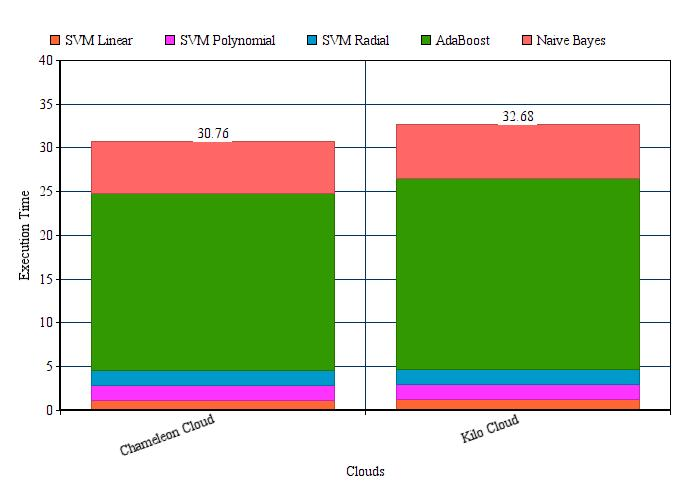
\includegraphics[width=60mm,height=60mm]{images/algo_comparison.jpg}}
\caption{fig: Graph plot of algorithm execution time on chameleon and kilo clouds}
\label{fig: Graph plot of algorithm execution time on chameleon and kilo clouds}
\end{figure}

Further, the stopwatch command on CMD5 module was used to benchmark
execution time of kubernetes cluster creation, software deployment and
installation on both chameleon and kilo cloud. By segmenting the
all-round application runtime into software installation, cluster
creation and code deployment we can clearly observe the performance of
the cluster on each cloud.


\section{Discussion}
TBD

\section{Conclusion}

TBD

\section{Acknowledgement}

We acknowledge our professor Gregor von Laszewski and all associate
instructors for helping us and guiding us throughout this project.

\section{Appendices}
TBD

% Bibliography

\bibliography{references} 

\end{document}
